\documentclass{beamer} % default... %
%\documentclass[notes=only]{beamer} % notes only %
\usetheme{metropolis}

\usepackage{graphicx}
\usepackage{hyperref}
%\usepackage{listings}
\usepackage{minted}

\graphicspath{{figures/}}

%\usepackage{fontspec}
%\setsansfont{Ubuntu}
%\setmonofont{Ubuntu Mono}

%%%% some of my lkurusa-tools %%%%

\newcommand*{\emailify}[1]{$<$#1$>$}
\newcommand*{\myemail}{\emailify{lkurusa@linux.com}}
\newcommand*{\ptrace}{\texttt{ptrace}}
\newcommand*{\ptraceman}{\texttt{ptrace(2)}}

%%%%%%%%

\title{Let's write a Debugger!}
\author{Levente Kurusa \myemail}
\date{Imperial College London}
\institute{\texttt{linux.conf.au 2018}, Sydney, Australia \hfill January 25, 2018}

\begin{document}
\maketitle

\begin{frame}{Who am I?}
\begin{itemize}
  \item Final year undergraduate at Imperial College London
  \item Previously at Apple and Red Hat
  \item Now researching different ways of operating system construction
  \item Low-level hacker
\end{itemize}
\end{frame}

\section{History of debuggers}

\begin{frame}{Single user machines}

\begin{columns}
\column{0.5\textwidth}
\begin{itemize}
    \item One of the first computers in the world
    \item Small application was loaded at the top of the memory
      \begin{itemize}
          \item single step
          \item examine registers
          \item read/write memory
      \end{itemize}
\end{itemize}

\column{0.5\textwidth}
\metroset{block=fill}
\begin{block}{TX-0 at MIT}
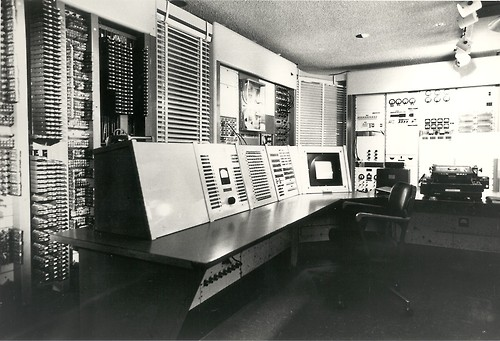
\includegraphics[width=0.4\paperwidth]{tx0.jpg}
\end{block}

\end{columns}

\note{
    Prepunched cards with the code\\
    Names like DDT and ODT
}

\end{frame}

\begin{frame}{Batch processing machines}
\includegraphics<1>[width=\textwidth]{punch_card_stack.jpg}
%TODO: https://en.wikipedia.org/wiki/Punched_card#/media/File:Punched_card_program_deck.agr.jpg
%TODO: Mention license at the end and attribute
\pause
Debugged by putting macro call in the punch card and generating:
\begin{itemize}
    \item Snapshots \textit{(register dump)}
    \item Core dumps \textit{(contents of memory)}
\end{itemize}

\note{
    A different class of machines was also on the rise. \\
    Submit a stack of punch cards and wait for the result at the end of the day
}

\end{frame}

\begin{frame}[fragile]
\frametitle{printf}

Then came CTSS \textit{(Compatible Time-Sharing System)}, one of the first time-sharing operating
systems! \par
\vspace{.5cm}
Debugging suddenly became interactive.

\metroset{block=fill}
\begin{block}{printf-debugging}
\begin{minted}{c}
  *ptr = 1337;
  printf("Did we crash at line %d?\n", __LINE__);
  *((int *) 0) = 1337;
  printf("Did we crash at line %d?\n", __LINE__);
\end{minted}
\end{block}

\end{frame}

\begin{frame}{Unix-es}
\begin{itemize}
    \item The first version of Unix had a debugger called, \texttt{DB}
    \item GNU had \texttt{GDB} and \texttt{LLDB}
    \item For Plan 9, \texttt{ADB} was created
\end{itemize}
\vskip.5cm
These debuggers should be familiar!
\end{frame}

\section{Tracing processes}

\begin{frame}[fragile]
\frametitle{ptrace}

Most debuggers heavily rely on a system call known as \ptrace.
\vskip1cm
\metroset{block=fill}
\begin{block}{The prototype of \ptraceman}
\begin{minted}{c}
#include <sys/ptrace.h>

long ptrace(enum __ptrace_request request, pid_t pid,
                   void *addr, void *data);
\end{minted}
\end{block}
\end{frame}

\begin{frame}{Signals}
Signals originate from CPU exceptions..
\end{frame}

\begin{frame}{Implementation}
\begin{itemize}[<+- | alert@+>]
    \item<1-> \alert<2>{Enable tracing}
    \item<1-> \alert<3>{Run until system call}
    \item<1-> \alert<4>{Monitoring registers}
    \item<1-> \alert<5>{Single stepping}
\end{itemize}
\end{frame}

\section{Architectural support}

\begin{frame}{Interrupting a process}

\texttt{PTRACE\_SYSCALL} \\
\texttt{PTRACE\_SINGLESTEP}

Undefined instructions, debug interrupt...

\end{frame}

\begin{frame}{Debug registers}
\texttt{DR0-DR7}
\end{frame}

\begin{frame}{Thanks!}
\begin{center}
Thank you for your attention! \par
\end{center}

Twitter: @iLevex \hfill Email: \myemail \\
GitHub: levex \hfill Website: \url{http://osdev.me/}

\vspace{1cm}

\begin{small}
The \LaTeX\hskip1mm theme is available at \url{github.com/matze/mtheme}

The theme is licensed under a
\href{http://creativecommons.org/licenses/by-sa/4.0/}{CC-BY-SA 4.0 International license},
and the talk is licensed under the \href{https://opensource.org/licenses/MIT}{MIT license}.

\end{small}

\end{frame}

\end{document}
